\documentclass{standalone}
\usepackage{tikz}
\usetikzlibrary{patterns, positioning}


\begin{document}
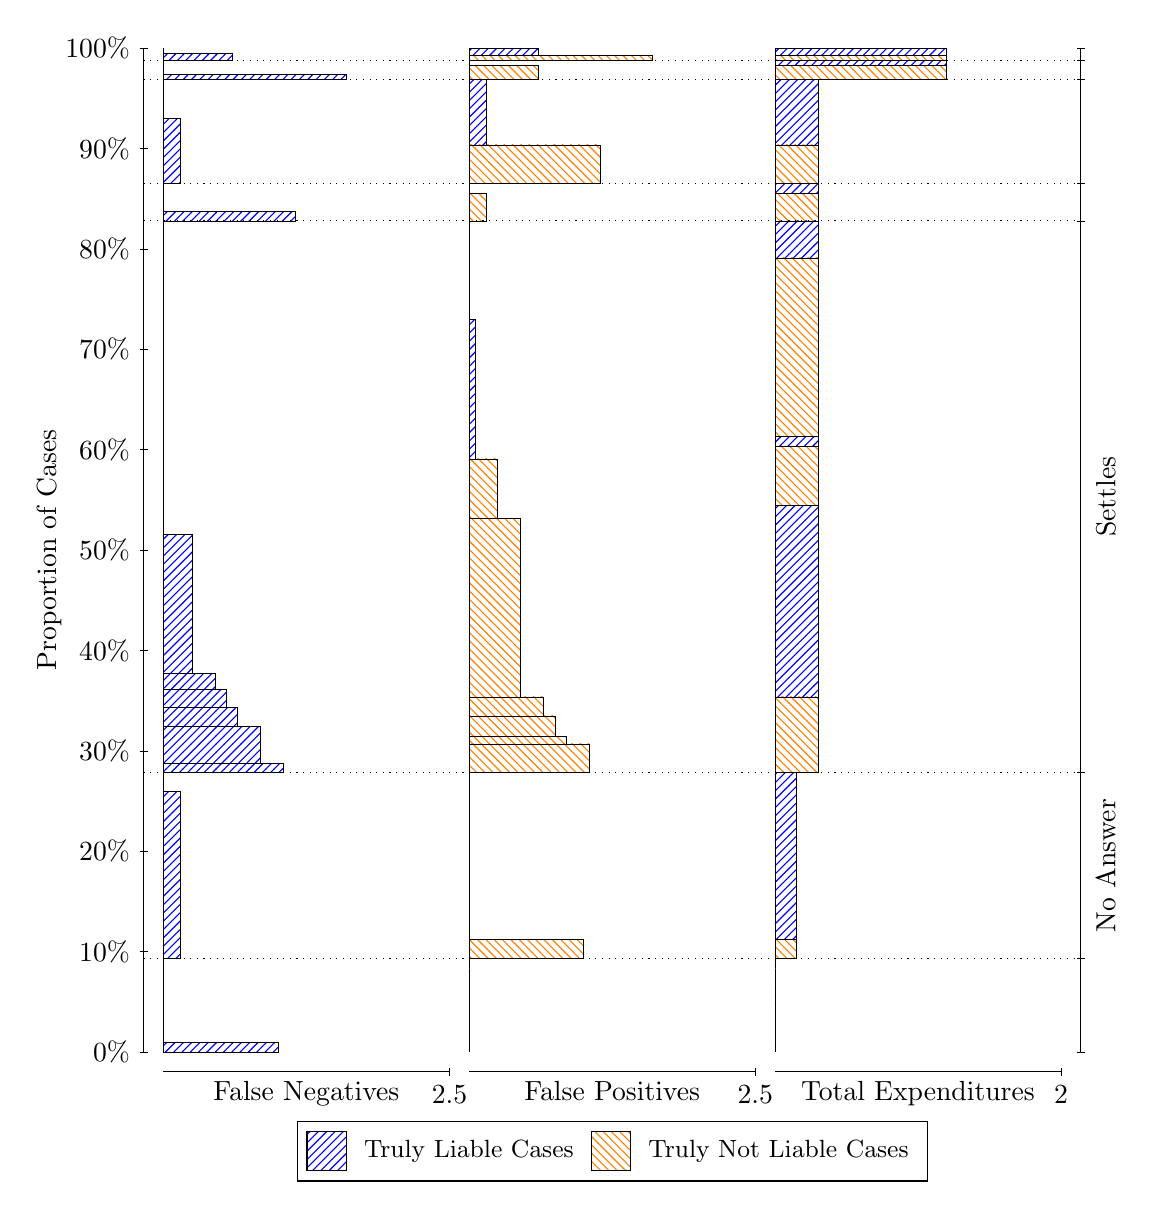
\begin{tikzpicture}
\draw[black, very thin] (1.5,1.75) -- (1.5,14.5);
\node[rotate=90, text=black, anchor=center] at (0.3, 8.125) {Proportion of Cases};
\draw[black, very thin] (1.45,1.75) -- (1.55,1.75);
\node[text=black, anchor=east] at (1.45, 1.75) {0\%};
\draw[black, very thin] (1.45,3.025) -- (1.55,3.025);
\node[text=black, anchor=east] at (1.45, 3.025) {10\%};
\draw[black, very thin] (1.45,4.3) -- (1.55,4.3);
\node[text=black, anchor=east] at (1.45, 4.3) {20\%};
\draw[black, very thin] (1.45,5.575) -- (1.55,5.575);
\node[text=black, anchor=east] at (1.45, 5.575) {30\%};
\draw[black, very thin] (1.45,6.85) -- (1.55,6.85);
\node[text=black, anchor=east] at (1.45, 6.85) {40\%};
\draw[black, very thin] (1.45,8.125) -- (1.55,8.125);
\node[text=black, anchor=east] at (1.45, 8.125) {50\%};
\draw[black, very thin] (1.45,9.4) -- (1.55,9.4);
\node[text=black, anchor=east] at (1.45, 9.4) {60\%};
\draw[black, very thin] (1.45,10.675) -- (1.55,10.675);
\node[text=black, anchor=east] at (1.45, 10.675) {70\%};
\draw[black, very thin] (1.45,11.95) -- (1.55,11.95);
\node[text=black, anchor=east] at (1.45, 11.95) {80\%};
\draw[black, very thin] (1.45,13.225) -- (1.55,13.225);
\node[text=black, anchor=east] at (1.45, 13.225) {90\%};
\draw[black, very thin] (1.45,14.5) -- (1.55,14.5);
\node[text=black, anchor=east] at (1.45, 14.5) {100\%};

\draw[black, very thin] (13.4,1.75) -- (13.4,14.5);
\draw[black, very thin] (13.35,1.75) -- (13.45,1.75);
\node[anchor=west] at (13.35, 1.75) {};
\draw[black, very thin] (13.35,2.9362) -- (13.45,2.9362);
\node[anchor=west] at (13.35, 2.9362) {};
\draw[black, very thin] (13.35,5.2999) -- (13.45,5.2999);
\node[anchor=west] at (13.35, 5.2999) {};
\draw[black, very thin] (13.35,12.305) -- (13.45,12.305);
\node[anchor=west] at (13.35, 12.305) {};
\draw[black, very thin] (13.35,12.78) -- (13.45,12.78);
\node[anchor=west] at (13.35, 12.78) {};
\draw[black, very thin] (13.35,14.097) -- (13.45,14.097);
\node[anchor=west] at (13.35, 14.097) {};
\draw[black, very thin] (13.35,14.343) -- (13.45,14.343);
\node[anchor=west] at (13.35, 14.343) {};
\draw[black, very thin] (13.35,14.5) -- (13.45,14.5);
\node[anchor=west] at (13.35, 14.5) {};

\draw[black, very thin, pattern color=blue, pattern=north east lines] (1.75,1.75) rectangle (3.2033,1.8748);
\draw[black, very thin, pattern color=orange, pattern=north west lines] (1.75,1.8748) rectangle (1.75,2.9362);
\draw[black, very thin, pattern color=blue, pattern=north east lines] (1.75,2.9362) rectangle (1.968,5.0546);
\draw[black, very thin, pattern color=orange, pattern=north west lines] (1.75,5.0546) rectangle (1.75,5.2999);
\draw[black, very thin, pattern color=blue, pattern=north east lines] (1.75,5.2999) rectangle (3.276,5.4193);
\draw[black, very thin, pattern color=blue, pattern=north east lines] (1.75,5.4193) rectangle (2.9853,5.889);
\draw[black, very thin, pattern color=blue, pattern=north east lines] (1.75,5.889) rectangle (2.6947,6.1303);
\draw[black, very thin, pattern color=blue, pattern=north east lines] (1.75,6.1303) rectangle (2.5493,6.3511);
\draw[black, very thin, pattern color=blue, pattern=north east lines] (1.75,6.3511) rectangle (2.404,6.5547);
\draw[black, very thin, pattern color=blue, pattern=north east lines] (1.75,6.5547) rectangle (2.1133,8.3233);
\draw[black, very thin, pattern color=orange, pattern=north west lines] (1.75,8.3233) rectangle (1.75,12.305);
\draw[black, very thin, pattern color=blue, pattern=north east lines] (1.75,12.305) rectangle (3.4213,12.429);
\draw[black, very thin, pattern color=orange, pattern=north west lines] (1.75,12.429) rectangle (1.75,12.78);
\draw[black, very thin, pattern color=blue, pattern=north east lines] (1.75,12.78) rectangle (1.968,13.608);
\draw[black, very thin, pattern color=orange, pattern=north west lines] (1.75,13.608) rectangle (1.75,14.097);
\draw[black, very thin, pattern color=blue, pattern=north east lines] (1.75,14.097) rectangle (4.0753,14.161);
\draw[black, very thin, pattern color=orange, pattern=north west lines] (1.75,14.161) rectangle (1.75,14.343);
\draw[black, very thin, pattern color=blue, pattern=north east lines] (1.75,14.343) rectangle (2.622,14.436);
\draw[black, very thin, pattern color=orange, pattern=north west lines] (1.75,14.436) rectangle (1.75,14.5);
\draw[black, very thin, pattern color=orange, pattern=north west lines] (5.6333,1.75) rectangle (5.6333,2.8114);
\draw[black, very thin, pattern color=blue, pattern=north east lines] (5.6333,2.8114) rectangle (5.6333,2.9362);
\draw[black, very thin, pattern color=orange, pattern=north west lines] (5.6333,2.9362) rectangle (7.0867,3.1815);
\draw[black, very thin, pattern color=blue, pattern=north east lines] (5.6333,3.1815) rectangle (5.6333,5.2999);
\draw[black, very thin, pattern color=orange, pattern=north west lines] (5.6333,5.2999) rectangle (7.1593,5.6624);
\draw[black, very thin, pattern color=orange, pattern=north west lines] (5.6333,5.6624) rectangle (6.8687,5.7546);
\draw[black, very thin, pattern color=orange, pattern=north west lines] (5.6333,5.7546) rectangle (6.7233,6.017);
\draw[black, very thin, pattern color=orange, pattern=north west lines] (5.6333,6.017) rectangle (6.578,6.2583);
\draw[black, very thin, pattern color=orange, pattern=north west lines] (5.6333,6.2583) rectangle (6.2873,8.5273);
\draw[black, very thin, pattern color=orange, pattern=north west lines] (5.6333,8.5273) rectangle (5.9967,9.282);
\draw[black, very thin, pattern color=blue, pattern=north east lines] (5.6333,9.282) rectangle (5.706,11.051);
\draw[black, very thin, pattern color=blue, pattern=north east lines] (5.6333,11.051) rectangle (5.6333,12.305);
\draw[black, very thin, pattern color=orange, pattern=north west lines] (5.6333,12.305) rectangle (5.8513,12.657);
\draw[black, very thin, pattern color=blue, pattern=north east lines] (5.6333,12.657) rectangle (5.6333,12.78);
\draw[black, very thin, pattern color=orange, pattern=north west lines] (5.6333,12.78) rectangle (7.3047,13.269);
\draw[black, very thin, pattern color=blue, pattern=north east lines] (5.6333,13.269) rectangle (5.8513,14.097);
\draw[black, very thin, pattern color=orange, pattern=north west lines] (5.6333,14.097) rectangle (6.5053,14.279);
\draw[black, very thin, pattern color=blue, pattern=north east lines] (5.6333,14.279) rectangle (5.6333,14.343);
\draw[black, very thin, pattern color=orange, pattern=north west lines] (5.6333,14.343) rectangle (7.9587,14.407);
\draw[black, very thin, pattern color=blue, pattern=north east lines] (5.6333,14.407) rectangle (6.5053,14.5);
\draw[black, very thin, pattern color=orange, pattern=north west lines] (9.5167,1.75) rectangle (9.5167,2.8114);
\draw[black, very thin, pattern color=blue, pattern=north east lines] (9.5167,2.8114) rectangle (9.5167,2.9362);
\draw[black, very thin, pattern color=orange, pattern=north west lines] (9.5167,2.9362) rectangle (9.7892,3.1815);
\draw[black, very thin, pattern color=blue, pattern=north east lines] (9.5167,3.1815) rectangle (9.7892,5.2999);
\draw[black, very thin, pattern color=orange, pattern=north west lines] (9.5167,5.2999) rectangle (10.062,6.2583);
\draw[black, very thin, pattern color=blue, pattern=north east lines] (9.5167,6.2583) rectangle (10.062,8.6926);
\draw[black, very thin, pattern color=orange, pattern=north west lines] (9.5167,8.6926) rectangle (10.062,9.4473);
\draw[black, very thin, pattern color=blue, pattern=north east lines] (9.5167,9.4473) rectangle (10.062,9.5667);
\draw[black, very thin, pattern color=orange, pattern=north west lines] (9.5167,9.5667) rectangle (10.062,11.836);
\draw[black, very thin, pattern color=blue, pattern=north east lines] (9.5167,11.836) rectangle (10.062,12.305);
\draw[black, very thin, pattern color=orange, pattern=north west lines] (9.5167,12.305) rectangle (10.062,12.657);
\draw[black, very thin, pattern color=blue, pattern=north east lines] (9.5167,12.657) rectangle (10.062,12.78);
\draw[black, very thin, pattern color=orange, pattern=north west lines] (9.5167,12.78) rectangle (10.062,13.269);
\draw[black, very thin, pattern color=blue, pattern=north east lines] (9.5167,13.269) rectangle (10.062,14.097);
\draw[black, very thin, pattern color=orange, pattern=north west lines] (9.5167,14.097) rectangle (11.697,14.279);
\draw[black, very thin, pattern color=blue, pattern=north east lines] (9.5167,14.279) rectangle (11.697,14.343);
\draw[black, very thin, pattern color=orange, pattern=north west lines] (9.5167,14.343) rectangle (11.697,14.407);
\draw[black, very thin, pattern color=blue, pattern=north east lines] (9.5167,14.407) rectangle (11.697,14.5);
\draw[black, dotted] (1.5,2.9362) -- (13.4,2.9362);
\draw[black, dotted] (1.5,5.2999) -- (13.4,5.2999);
\draw[black, dotted] (1.5,12.305) -- (13.4,12.305);
\draw[black, dotted] (1.5,12.78) -- (13.4,12.78);
\draw[black, dotted] (1.5,14.097) -- (13.4,14.097);
\draw[black, dotted] (1.5,14.343) -- (13.4,14.343);
\draw[black, very thin] (1.75,1.5) -- (5.3833,1.5);
\node[text=black, anchor=north] at (3.5667, 1.5) {False Negatives};
\draw[black, very thin] (5.3833,1.45) -- (5.3833,1.55);
\node[text=black, anchor=north] at (5.3833, 1.45) {2.5};

\draw[black, very thin] (5.6333,1.5) -- (9.2667,1.5);
\node[text=black, anchor=north] at (7.45, 1.5) {False Positives};
\draw[black, very thin] (9.2667,1.45) -- (9.2667,1.55);
\node[text=black, anchor=north] at (9.2667, 1.45) {2.5};

\draw[black, very thin] (9.5167,1.5) -- (13.15,1.5);
\node[text=black, anchor=north] at (11.333, 1.5) {Total Expenditures};
\draw[black, very thin] (13.15,1.45) -- (13.15,1.55);
\node[text=black, anchor=north] at (13.15, 1.45) {2};


\node[text=black, centered, rotate=90] at (13.72, 4.118) {No Answer};
\node[text=black, centered, rotate=90] at (13.72, 8.8027) {Settles};





\draw (7.449999999999999,1.5) node[draw=none] (baseCoordinate) {};
\begin{scope}[align=center]
        \matrix[scale=0.5, draw=black, below=0.5cm of baseCoordinate, nodes={draw}, column sep=0.1cm]{
            \node[rectangle, draw, minimum width=0.5cm, minimum height=0.5cm, pattern color=blue, pattern=north east lines] {}; &
            \node[draw=none, font=\small, text=black] (B) {Truly Liable Cases}; &
            \node[rectangle, draw, minimum width=0.5cm, minimum height=0.5cm, pattern color=orange, pattern=north west lines] {}; &
            \node[draw=none, font=\small, text=black] (B) {Truly Not Liable Cases}; \\
            };
\end{scope}

\end{tikzpicture}
\end{document}